\chapter{Aplicación Smart-Traffic-Sensor para Monitorización de Tráfico Rodado}\label{cap.diseno}

En este capítulo se hace una descripción del sistema desarrollado para llevar a cabo la monitorización visual de vehículos.

\section{Bases de Datos de Entrenamiento}\label{sec.base_datos}

Dado que queremos encontrar los vehículos en cuestión bajo diferentes circunstancias, es decir, en diferentes entornos y con diferentes iluminaciones, necesitaremos entrenar el modelo neuronal con un conjunto de imágenes representativo. Por este motivo, a lo largo de los últimos años han surgido diferentes \textit{datasets} públicos con el fin de permitir el entrenamiento de redes neuronales. Para el caso de la detección de vehículos hay pocos \textit{datasets}, por ello ha sido necesario crear una base de datos propia que tuviera un número suficiente de muestras y una variación amplia de tipos de escenarios, de vehículos, condiciones de luz, etc.

Inicialmente se creó una base de datos de menor tamaño, denominada \textit{Dataset STS}. Este \textit{dataset} incluía 3476 imágenes todas ellas de buena calidad y en buenas condiciones meteorológicas, las cuales se obtuvieron en su mayoría de la base de datos recopilada por Redouane Kachach en su tesis doctoral~\cite{traffic_monitor_lab}. De las 3476, 3173 se asignaron al entrenamiento de la red neuronal y 303 a test. Además, esas 3173 imágenes, contienen 2700 de \textit{train} y 473 de validación.

La distribución de las muestras que poseen las imágenes empleadas para el entrenamiento (3173 imágenes) se indica en la Tabla~\ref{tabla_database}.

\begin{table}[H]
\begin{center}
\begin{tabular}{|l|l|}
\hline
Clases & Muestras \\
\hline \hline
Car & 15798 \\ \hline
Motorcycle & 143 \\ \hline
Van & 1437 \\ \hline
Bus & 274 \\ \hline
Truck & 765 \\ \hline
Small-Truck & 400 \\ \hline
Tank-Truck & 103 \\ \hline
Total & 18920 \\ \hline
\end{tabular}
\caption{\textit{Dataset STS}. Imágenes para el Entrenamiento}
\label{tabla_database}
\end{center}
\end{table}

Tal y como ya se ha dicho, de las 3476 imágenes del \textit{Dataset STS}, 303 eran de test. En la Tabla~\ref{tabla_datos_primera_evaluacion} se puede ver qué clases de muestras contenían las imágenes de test.

\begin{table}[H]
\begin{center}
\begin{tabular}{|l|l|}
\hline
Clases & Muestras \\
\hline \hline
Car & 922 \\ \hline
Motorcycle & 19 \\ \hline
Van & 125 \\ \hline
Truck & 82 \\ \hline
Small-Truck & 112 \\ \hline
Total & 1260 \\ \hline
\end{tabular}
\caption{\textit{Dataset STS}. Imágenes de Test}
\label{tabla_datos_primera_evaluacion}
\end{center}
\end{table}

Para intentar conseguir un sistema robusto ante diferentes condiciones, se amplió la base de datos incluyendo imágenes en condiciones meteorológicas buenas, imágenes en condiciones meteorológicas malas (con niebla y lluvia) e imágenes de mala calidad. Al hacernos con más imágenes recopiladas de diferentes fuentes se creó una base de datos de mayor tamaño denominada \textit{Dataset STS Enriquecido}. Esta base de datos propia consta de:
\begin{itemize}
    \item La base de datos recopilada por Redouane Kachach en su tesis doctoral, para la aplicación \textit{TrafficMonitor}, que es antecesor directo de este TFM~\cite{traffic_monitor_lab}. Dicha base de datos consta de 3460 imágenes de buena calidad.
    \item La base de datos \acrfull{gram} creada por R. Guerrero-Gomez-Olmedo, R. J. Lopez-Sastre, S. Maldonado-Bascon and A. Fernandez-Caballero~\cite{guerrero2013iwinac}. Esta base de datos está formada por imágenes extraídas de tres vídeos. El primer vídeo, llamado M-30 (7520 fotogramas), se grabó en un día soleado. El segundo, llamado M-30-HD (9390 fotogramas), se grabó en una ubicación similar pero durante un día nublado. El tercero, llamado Urban1 (23435 fotogramas) se grabó en una intersección concurrida. De esta gran base de datos se emplearon 3646 imágenes del vídeo M-30-HD y 1348 del vídeo M-30.
    \item Imágenes recopiladas de cámaras en abierto de forma online durante este TFM. 615 se trataban de situaciones de lluvia y 705 de imágenes con mala calidad.
\end{itemize} 

Se ha tratado que la base de datos construida abarcara la mayor diversidad de vehículos posibles y en diferente tipos de escenarios. Hay que tener en cuenta que toda la base de datos tiene vehículos vistos por la parte trasera. En total consta de 9774 imágenes y está formada por 7 clases: \textit{Car}, \textit{Motorcycle}, \textit{Van}, \textit{Bus}, \textit{Truck}, \textit{Small-truck} y \textit{Tank-truck}.


En estas 9774 imágenes tenemos un total de 48914 muestras repartidas tal y como se muestra en la Tabla~\ref{tabla_muestras}.

\begin{table}[htbp] 
\begin{center}
\begin{tabular}{|l|l|}
\hline
Clases & Muestras \\
\hline \hline
Car & 38976 \\ \hline
Motorcycle & 1886 \\ \hline
Van & 5631 \\ \hline
Bus & 401 \\ \hline
Truck & 963 \\ \hline
Small-Truck & 938 \\ \hline
Tank-Truck & 119 \\ \hline
\end{tabular}
\caption{Muestras de la Base de Datos \textit{Dataset STS Enriquecido}}
\label{tabla_muestras}
\end{center}
\end{table}

Tal y como se ha dicho anteriormente la base de datos \textit{Dataset STS Enriquecido} contiene imágenes de buena calidad, de condiciones climatológicas adversas y de mala calidad. En la Tabla ~\ref{tabla_img_base_datos} se puede ver la cantidad de imágenes que hay para cada tipo.

\begin{table}[htb]
\begin{center}
\begin{tabular}{|l|l|}
\hline
\cline{2-2}& Nº de Imágenes\\
\hline \hline
Buena calidad & 8406 \\ \hline
Malas Condiciones Meteorológicas & 663\\ \hline
Mala Calidad & 705\\ \hline
\end{tabular}
\caption{Imágenes de \textit{Dataset STS Enriquecido}}
\label{tabla_img_base_datos}
\end{center}
\end{table}

En la Figura~\ref{fig.base_datos} se pueden ver algunas imágenes de nuestra base de datos.

\begin{figure}[H]
\begin{center}
	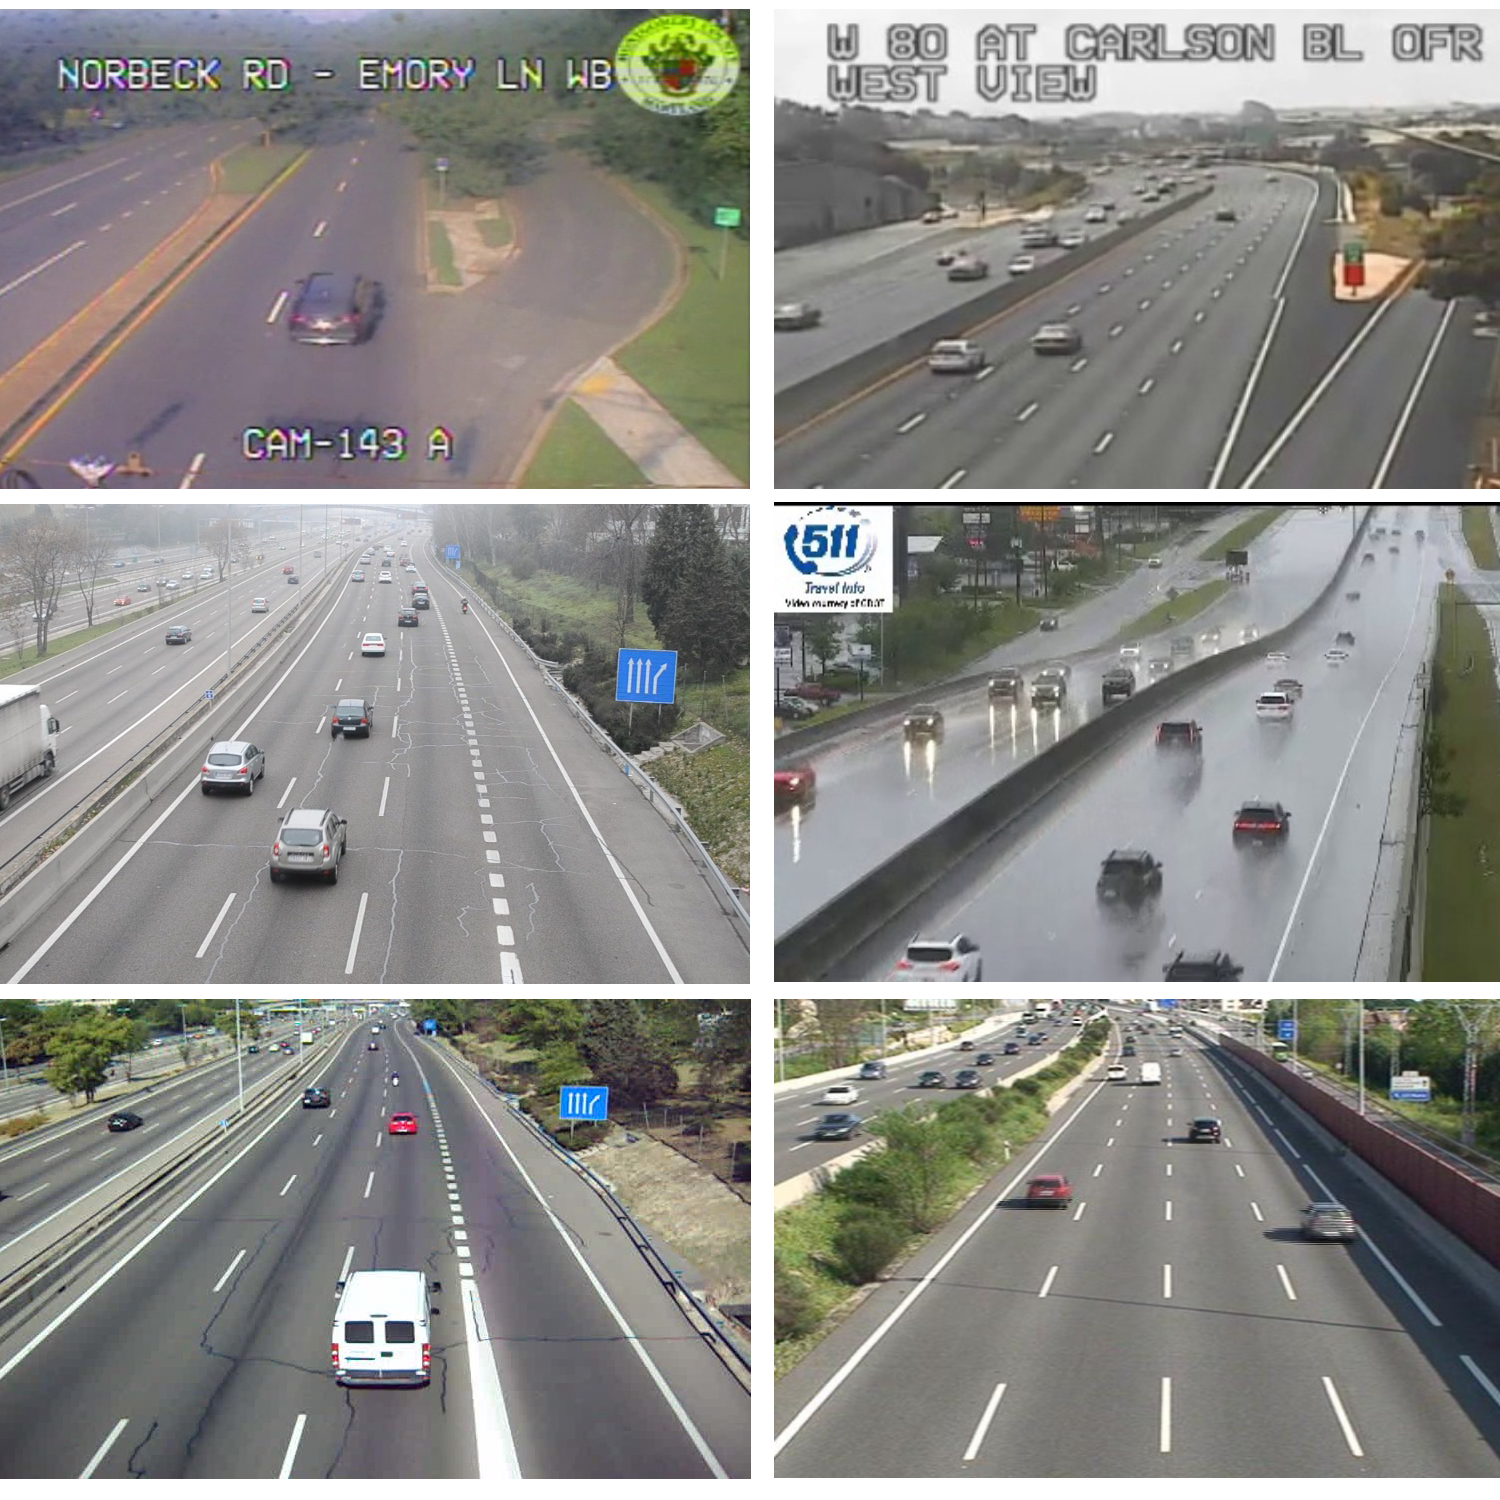
\includegraphics[width=0.6\textwidth]{figures/Diseno_global/base_datos.png}
   \caption{\textit{Dataset STS Enriquecido}}
	\label{fig.base_datos}
\end{center}
\end{figure}

De estas 9774 imágenes una parte se empleó en el entrenamiento y otra en el test. En la Tabla~\ref{tabla_distribucion_base_datos} se muestra la distribución de imágenes en función de \textit{train} y test.

\begin{table}[H] 
\begin{center}
\begin{tabular}{|l|l|l|}
\hline
Tipo & Imágenes de Train & Imágenes de Test  \\ 
\hline \hline
Buena Calidad & 6717 & 389  \\ \hline
Malas Condiciones Meteorológicas & 1892 & 71 \\ \hline
Mala Calidad  & 637 & 68  \\ \hline
Total & 9246 & 528 \\ \hline
\end{tabular}
\caption{Distribución \textit{Dataset STS Enriquecido}}
\label{tabla_distribucion_base_datos}
\end{center}
\end{table}

Para el entrenamiento de la red neuronal la base de datos de entrenamiento se dividió en \textit{train} y validación. De las 9246 imágenes, 7401 se usaban como \textit{train} y 1845 como validación. En la Tabla~\ref{base_datos_final_train} se puede observar la cantidad de imágenes que se han empleado en el entrenamiento en función de su tipo (buena calidad, mala calidad y condiciones meteorológicas desfavorables).

\begin{table}[H]
\begin{center}
\begin{tabular}{|l|l|l|l|}
\hline
Tipo  & Imágenes de Train & Imágenes de Validación & Total \\
\hline \hline
Buena Calidad & 5323 &  1394 & 6717 \\ \hline
Condiciones Meteorológicas malas & 1568 & 324 & 1892 \\ \hline
Mala Calidad & 510 & 127 & 637 \\ \hline
Total & 7401 & 1845 & 9246 \\ \hline
\end{tabular}
\caption{\textit{Dataset STS Enriquecido} de Entrenamiento}
\label{base_datos_final_train}
\end{center}
\end{table}

La cantidad de muestras de cada clase que tienen las imágenes de buena calidad para el entrenamiento puede verse en la Tabla~\ref{tabla_redes_database_mayor}. 

\begin{table}[H]
\begin{center}
\begin{tabular}{|l|l|}
\hline
Clases & Muestras \\
\hline \hline
Car & 28655 \\ \hline
Motorcycle & 1517 \\ \hline
Van & 4675 \\ \hline
Bus & 274 \\ \hline
Truck & 874 \\ \hline
Small-Truck & 663 \\ \hline
Tank-Truck & 103 \\ \hline
Total & 36762 \\ \hline
\end{tabular}
\caption{Características de las Imágenes de Buena Calidad del \textit{Dataset STS Enriquecido} para el Entrenamiento}
\label{tabla_redes_database_mayor}
\end{center}
\end{table}

Los tipos de muestras que hay en las imágenes de malas condiciones climatológicas pueden verse en la Tabla~\ref{tabla_redes_database_malas_condiciones} y los de las imágenes de mala calidad en la Tabla~\ref{tabla_redes_database_mala_calidad}.

\begin{table}[H]
\begin{center}
\begin{tabular}{|l|l|}
\hline
Clases & Muestras \\
\hline \hline
Car & 6921 \\ \hline
Motorcycle & 335 \\ \hline
Van & 709 \\ \hline
Bus & 100 \\ \hline
Small-Truck & 183 \\ \hline
Total & 8248 \\ \hline
\end{tabular}
\caption{Características de las Imágenes de Condiciones Climatológicas Desfavorables del \textit{Dataset STS Enriquecido} para el Entrenamiento}
\label{tabla_redes_database_malas_condiciones}
\end{center}
\end{table}

\begin{table}[H]
\begin{center}
\begin{tabular}{|l|l|}
\hline
Clases & Muestras \\
\hline \hline
Car & 1571 \\ \hline
Motorcycle & 21 \\ \hline
Van & 56 \\ \hline
Bus & 27 \\ \hline
Truck & 82 \\ \hline
Small-Truck & 60 \\ \hline
Tank-truck & 16 \\ \hline
Total & 1833 \\ \hline
\end{tabular}
\caption{Características de las Imágenes de Mala Calidad del \textit{Dataset STS Enriquecido} para el Entrenamiento}
\label{tabla_redes_database_mala_calidad}
\end{center}
\end{table}

Las imágenes de test incluyen muestras de buena calidad, de malas condiciones climatológicas y de mala calidad. A continuación se muestra información acerca de cada tipo de conjunto.

En la Tabla~\ref{tab_img_test_buenas} se muestra información acerca de las imágenes de test de buena calidad.
\begin{table}[H] 
\begin{center}
\begin{tabular}{|l|l|}
\hline
Nº de Imágenes  & 389 \\
\hline \hline
Nº de Muestras Totales & 1657\\ \hline
Nº Car & 1463 \\ \hline
Nº Motorcycle & 9 \\ \hline
Nº Van & 155 \\ \hline
Nº Truck & 8 \\ \hline
Nº Small-Truck & 22 \\ \hline
\end{tabular}
\caption{Imágenes de Test de Buena Calidad de \textit{Dataset STS Enriquecido}}
\label{tab_img_test_buenas}
\end{center}
\end{table}

La Tabla~\ref{tab_img_test_malas_condiciones} nos da información acerca de las imágenes de test de malas condiciones meteorológicas empleadas en la evaluación.
\begin{table}[H] 
\begin{center}
\begin{tabular}{|l|l|}
\hline
Nº de Imágenes  & 71 \\
\hline \hline
Nº de Muestras Totales & 287\\ \hline
Nº Car & 263 \\ \hline
Nº Motorcycle & 1 \\ \hline
Nº Van & 23 \\ \hline
\end{tabular}
\caption{Imágenes de Test de Malas Condiciones Meteorológicas de \textit{Dataset STS Enriquecido}}
\label{tab_img_test_malas_condiciones}
\end{center}
\end{table}

El conjunto de imágenes de test con mala calidad queda caracterizado en la Tabla~\ref{tab_img_test_mala_calidad}.

\begin{table}[H] 
\begin{center}
\begin{tabular}{|l|l|}
\hline
Nº de Imágenes  & 68 \\
\hline \hline
Nº de Muestras Totales & 199\\ \hline
Nº Car & 176 \\ \hline
Nº Motorcycle & 3 \\ \hline
Nº Van & 11 \\ \hline
Nº Small-Truck & 9 \\ \hline
\end{tabular}
\caption{Imágenes de Test de Mala Calidad de \textit{Dataset STS Enriquecido}}
\label{tab_img_test_mala_calidad}
\end{center}
\end{table}


Hay que decir que todas las imágenes han sido etiquetadas a mano haciendo uso de la herramienta labelImg~\cite{labelimg}, la cual permite guardar las etiquetas en archivos xml, en formato PASCAL VOC (formato usado por ImageNet) o en formato \acrshort{yolo} en txt.

\section{Diseño de la Aplicación}

Nuestra aplicación es una especie de caja negra donde entran fotogramas de una secuencia de vídeo y salen dichas imágenes con los vehículos detectados e identificados en función del seguimiento y la clasificación. En la Figura~\ref{fig.caja_negra} se puede ver esta caja negra.

\begin{figure}[H] 
\begin{center}
	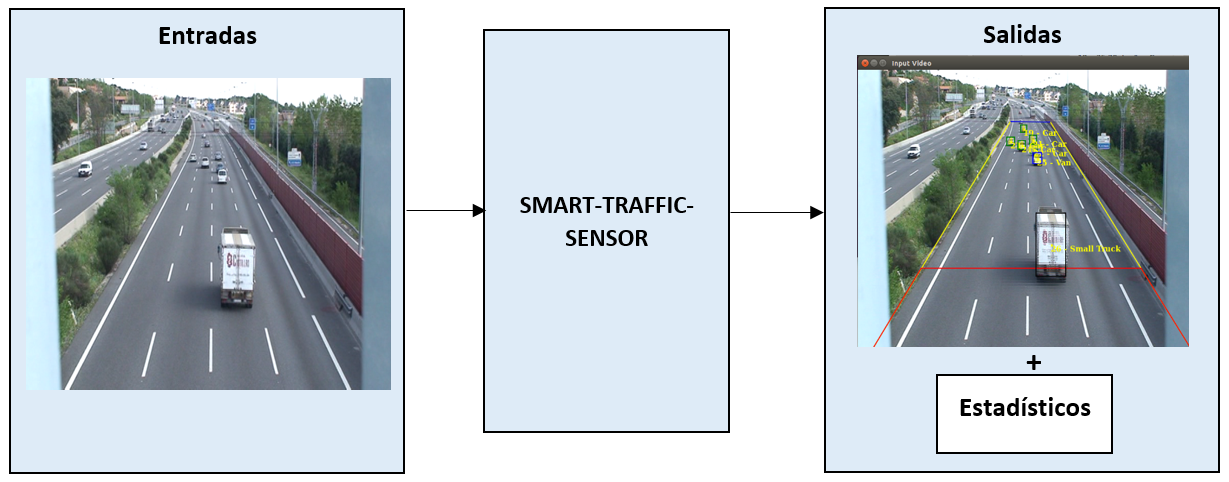
\includegraphics[width=1\textwidth]{figures/Diseno_global/caja_negra.PNG}
   \caption{Caja Negra}
	\label{fig.caja_negra}
\end{center}
\end{figure}

\textit{Smart-Traffic-Sensor} es un sistema que se realizó con el objetivo de monitorizar tráfico rodado en tiempo real. Esta monitorizacion consta de tres elementos principales:

\begin{itemize}
    \item Detección de vehículos
    \item Clasificación de vehículos
    \item Seguimiento de vehículos
\end{itemize}

En la Figura~\ref{fig.diagrama_bloques} se puede ver un diagrama de bloques que indica los elementos principales de los que se compone \textit{Smart-Traffic-Sensor}, es decir, en que se fundamenta para funcionar.

\begin{figure}
\begin{center}
	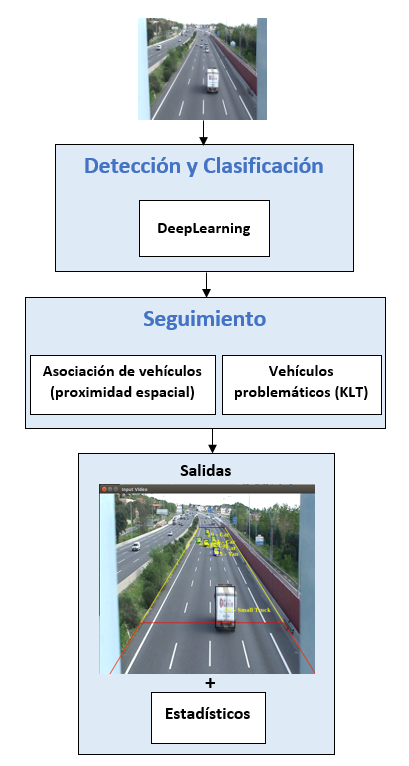
\includegraphics[width=0.5\textwidth]{figures/Diseno_global/diagrama_bloques.PNG}
   \caption{Diagrama de Bloques}
	\label{fig.diagrama_bloques}
\end{center}
\end{figure}

Las detecciones y la clasificación van de la mano, pues se realizan con \textit{Deep Learning}. En concreto con una red \acrshort{yolo}. Los vehículos que detectemos los clasificaremos en función a 7 clases:  \textit{car, motorcycle, van, bus, truck, small-truck} y \textit{tank-truck}. El seguimiento se centra en la proximidad espacial, y si ésta falla se utiliza \acrshort{klt}. A todos los \textit{blob} detectados se les realizará un seguimiento a lo largo del tiempo. 

El sistema del que partíamos (\textit{Traffic-Monitor}~\cite{traffic_monitor_redo}) definía en la imagen una zona de entrada y otra de seguimiento. Esto puede verse en la Figura ~\ref{fig.zonas}.

\begin{figure}[H] 
\begin{center}
	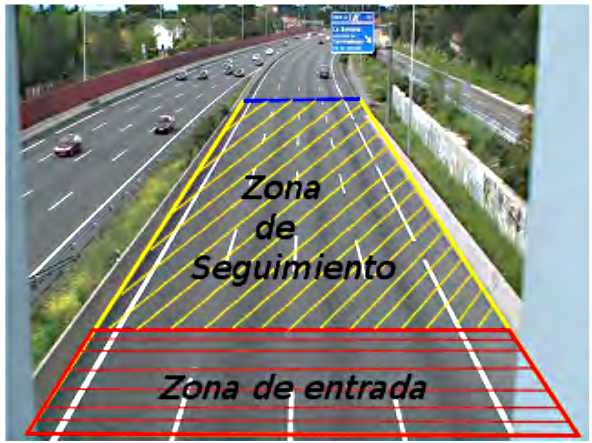
\includegraphics[width=0.5\textwidth]{figures/Diseno_global/zonas.jpg}
   \caption{Zonas de entrada y seguimiento}
	\label{fig.zonas}
\end{center}
\end{figure}

En la zona de entrada se realizan las detecciones y en la de seguimiento es donde se lleva a cabo la clasificación y el tracking de los vehículos.

Este concepto de separar zona de entrada y seguimiento va a perder relevancia en nuestro sistema, pues ya no va a ser necesario hacer esta distinción. Tendremos una única zona en la que se lleve a cabo la detección, la clasificación y el \textit{tracking}. Vamos a continuar teniendo una zona marcada en la imagen para identificar en qué parte de la carretera queremos centrar nuestras detecciones (por si existiesen carriles de diferente sentido). A esta zona de detección, clasificación y seguimiento vamos a llamarle zona de evaluación. En la Figura ~\ref{fig.nueva_zona} se puede ver la zona  de evaluación.

\begin{figure}[H] 
\begin{center}
	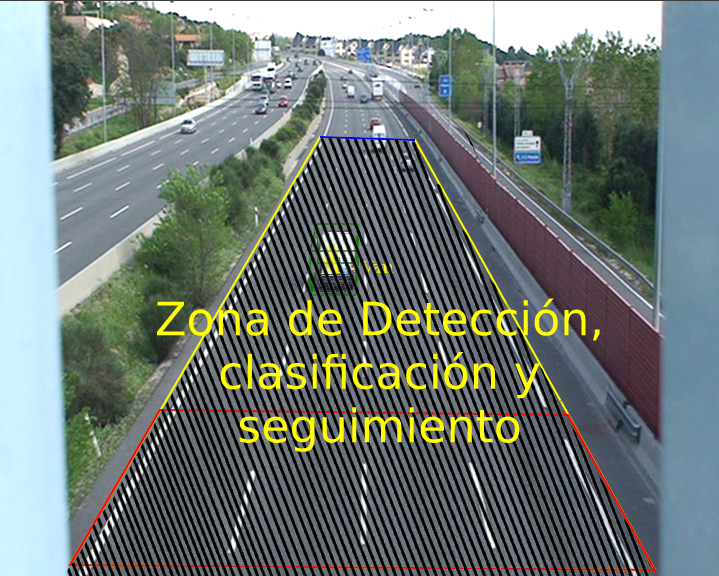
\includegraphics[width=0.5\textwidth]{figures/Diseno_global/nueva_zona.png}
   \caption{Zona Evaluación}
	\label{fig.nueva_zona}
\end{center}
\end{figure}


Este trabajo se ha basado principalmente en el uso de \textit{Deep Learning} para la clasificación y detección de vehículos. Además se ha apoyado en \acrfull{klt}, en los casos que pudiera haber pérdidas en la detección debido a oclusiones, o cuando los vehículos se encontraban muy alejados. Es decir, se ha apoyado en \acrshort{klt} cuando las condiciones a la hora de detectar eran algo complejas y por tanto el \textit{Deep Lerning} no era capaz de realizar correctamente la detección.

A la hora de realizar el \textit{tracking} se hace uso de la proximidad espacial, pero esto se explicará con más detalle en las siguientes secciones.


En resumen se puede decir que tenemos dos grandes bloques:
\begin{itemize}
    \item Detección y Clasificación de vehículos: para llevarlo a cabo se invoca a una red \acrshort{yolo} sobre la imagen completa. Dicha red fue entrenada con una base de datos propia de 9246 imágenes, las cuales fueron etiquetadas a mano.   
    \item Tracking de vehículos: se basa en la proximidad espacial para emparejar cada vehículo detectado con los vehículos detectados del instante anterior. Si un vehículo de los que está registrado no fuera detectado mediante \textit{Deep Learning} en el instante actual, se haría uso de \acrshort{klt} para estimar su posición. \acrshort{klt} permite determinar el movimiento de un objeto dentro de una secuencia de imágenes.
\end{itemize}

El conjunto total de detección, clasificación y seguimiento de vehículos tarda 50 ms, con lo cual se podría esperar que la aplicación funcione a unos 20 fotogramas por segundo. Las pruebas fueron realizadas mediante un servidor, por lo que el tiempo de actualización de los gráficos es mayor, obteniendo con ello que \textit{Smart-Traffic-Sensor} funcione a 10 fotogramas por segundo. No obstante esto debería probarse con un ordenador con GPU propia para ver realmente la velocidad a la que funciona. Todo esto se comentará más a fondo en el Capítulo \ref{cap.experimentos}.

A continuación se muestran dos diagramas de flujo, en los cuales se indica el planteamiento que se ha llevado a cabo en \textit{Smart-Traffic-Sensor}. En el primer diagrama~\ref{fig.diagrama_flujo_blob} se indica los pasos que se realizan una vez hemos detectado un \textit{blob} en la imagen. En el segundo~\ref{fig.diagrama_flujo_vehiculos} se muestra que es lo que se hace con los vehículos ya registrados, es decir, con los que se les está llevando un seguimiento.

\begin{figure}[H] 
\begin{center}
	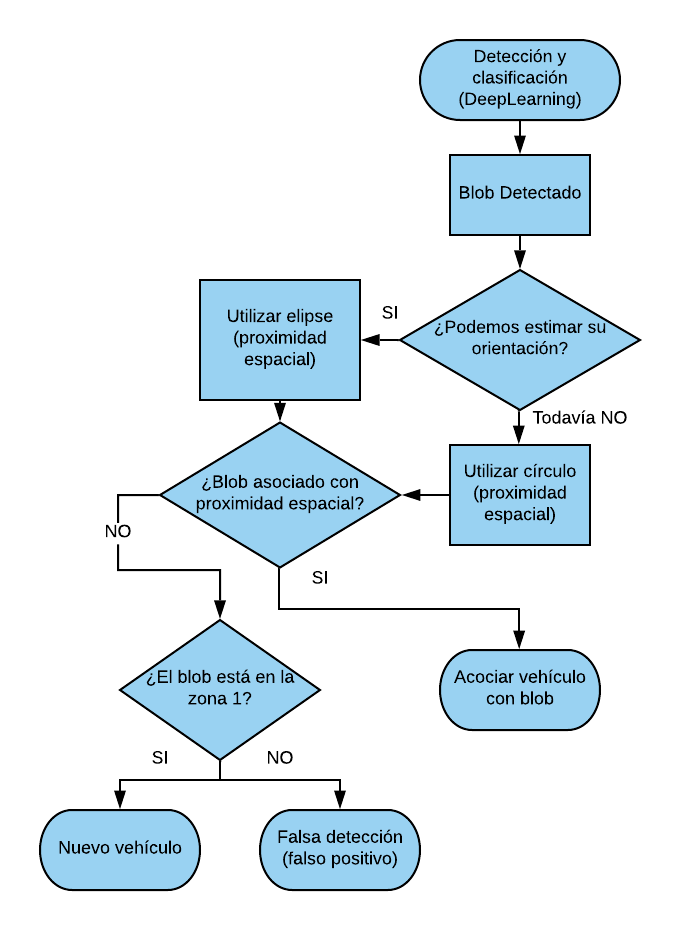
\includegraphics[width=0.8\textwidth]{figures/Diseno_global/diagrama_flujo.png}
   \caption{Diagrama de Flujo de  los Blobs Detectados}
	\label{fig.diagrama_flujo_blob}
\end{center}
\end{figure}

\begin{figure}[H] 
\begin{center}
	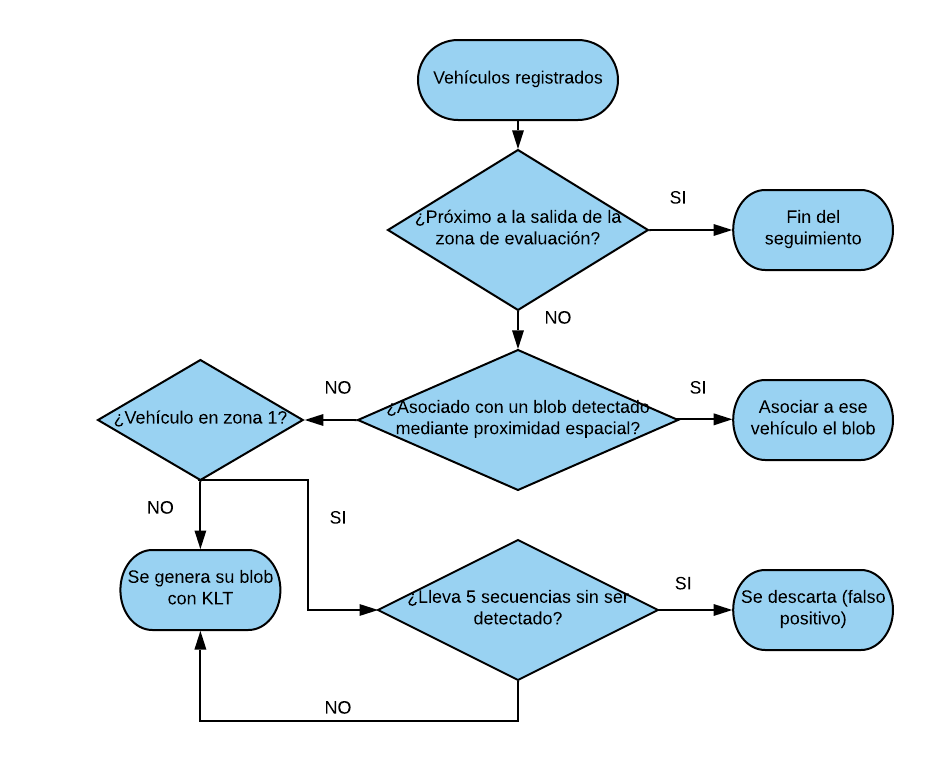
\includegraphics[width=0.9\textwidth]{figures/Diseno_global/diagrama_flujo1.png}
   \caption{Diagrama de Flujo de  los Vehículos Registrados}
	\label{fig.diagrama_flujo_vehiculos}
\end{center}
\end{figure}

\section{Detección y Clasificación}

Nuestro sistema toma como imágenes de entrada las adquiridas del vídeo que se esté monitorizando. Dichas imágenes pasan como entrada a la red neuronal, donde se detecta y clasifican los diversos vehículos. Toda la información se almacena en cada instante, para así poder realizar el tracking en función de la información registrada del instante anterior.

Tal y como ya se ha comentado anteriormente se ha hecho uso de \textit{Deep Learning}. En concreto se ha diseñado un sistema capaz de soportar redes neuronales entrenadas con diferentes \textit{frameworks} (\textit{TensorFlow}, \textit{Darknet} y \textit{Keras}) con el objetivo de detectar y clasificar los diferentes vehículos que aparezcan en la imagen. Con ello se ha pretendido realizar un sistema multiplataforma, el cual pueda adaptarse a los avances futuros de los diferentes entornos de \textit{Deep Learning}. Esto hace que nuestra aplicación no quede limitada ante la evolución de las redes neuronales.

En vídeos en carretera es muy probable que tengamos oclusiones y por supuesto vehículos que se vayan alejando, los cuales son bastante complejos de detectar. Para solventar esto nos hemos apoyado en \acrfull{klt}. Por tanto tenemos un sistema que complementa \textit{Deep Learning} con \acrshort{klt}. 

Para tener un sistema lo más robusto posible se han tenido en cuenta varios detalles:

\begin{itemize}
    \item Dentro de la zona de evaluación tenemos dos zonas. En la
     Figura ~\ref{fig.zona_evaluacion} quedan identificadas esas dos zonas.
    \begin{figure}[H] 
\begin{center}
	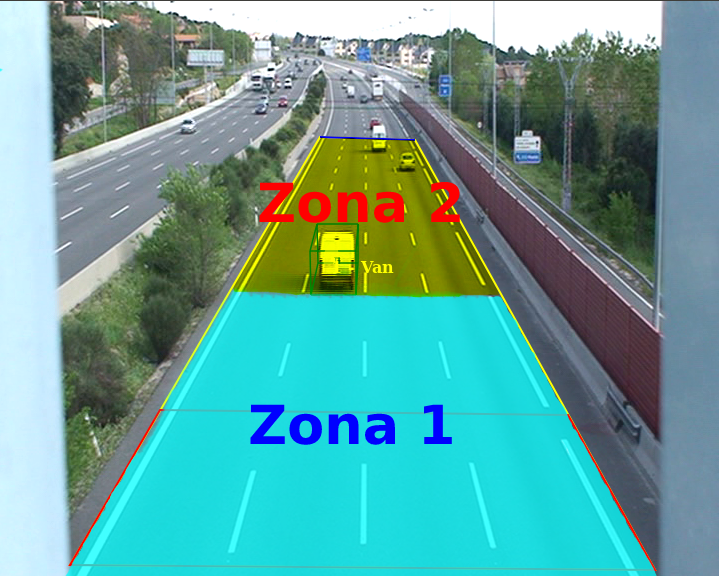
\includegraphics[width=0.7\textwidth]{figures/Diseno_global/zonas_evaluacion.png}
   \caption{Zonas identificadas en la zona de Evaluación}
	\label{fig.zona_evaluacion}
\end{center}

\end{figure}
    La zona 1 se corresponde con la mitad de la zona de evaluación por donde entran los vehículos. En esta zona es más sencillo detectar y clasificar los vehículos pues tienen mayor tamaño. La zona 2 hace referencia a la mitad por la que salen los vehículos, la cual es más compleja, pues los vehículos tendrán menor tamaño.
    \item Un vehículo siempre va a entrar a la zona de evaluación por la parte de entrada. Nunca puede aparecer de repente. Por ello no puede aparecer ningún vehículo nuevo en el medio de la carretera, es decir nunca se podrá estimar que se ha detectado un vehículo nuevo en la zona 2.
    \item Si en la zona 1 un vehículo no es detectado durante 5 secuencias seguidas se dará por hecho que ha sido un falso positivo y por tanto quedará descartado.
    \item Todo vehículo que se encuentre en la zona 2 se considerará que es un vehículo correcto. Si mediante \textit{Deep Learning} no somos capaces de detectar dicho vehículo, emplearemos \acrshort{klt} para localizarlo. 
\end{itemize}

En resumen, hay que tener en cuenta que no pueden aparecer vehículos nuevos en medio de la imagen, por tanto si esto sucede se considerará un falso positivo y se descartará. Otro aspecto que hay que tener en cuenta es que se podría dar una detección errónea, por ello si durante 5 secuencias seguidas un vehículo no ha sido detectado en la zona 1 se considerará como que era un falso positivo y se dejará de hacer su seguimiento.

Se han probado tres entornos diferentes para evaluar cual era el que mejores resultados obtenía. Para ello se hizo un primer entrenamiento con imágenes únicamente de buena calidad con el fin de determinar cual era el \textit{frameworks} que mejor funcionaba.


En los siguientes puntos se va a explicar el diseño que se ha llevado a cabo para integrar cada plataforma, en la aplicación \textit{Smart-Traffic-Sensor}.

\subsection{Entorno TensorFlow y red SSD MobilenetV2}\label{sub.tensorflow}

Para dar soporte dentro de la aplicación a redes de \textit{TensorFlow} se ha hecho uso del \textit{github models} de \textit{TensorFlow}~\cite{tensorflow_models}, con el cual podemos entrenar una red pre-entrenada con nuestra propia base de datos. En este caso se ha empleado una red \textit{\acrfull{ssd}} Mobilenet V2 entrenada con \acrshort{coco}, pues proporciona una buena relación entre la velocidad y la precisión. Para emplear dicha red se ha usado un archivo de configuración llamado \textit{ssd\_mobilenet\_v2\_coco.config}~\cite{ssd_mobilenetv2_config}.

La red \acrshort{ssd} MobileNet V2 es una red \acrshort{ssd} que en lugar de tener una red VGG-16 de base, tiene una red MobileNet. En la Figura ~\ref{fig.ssd_mobilenet} se puede ver dicho diseño.

\begin{figure}[H] 
\begin{center}
	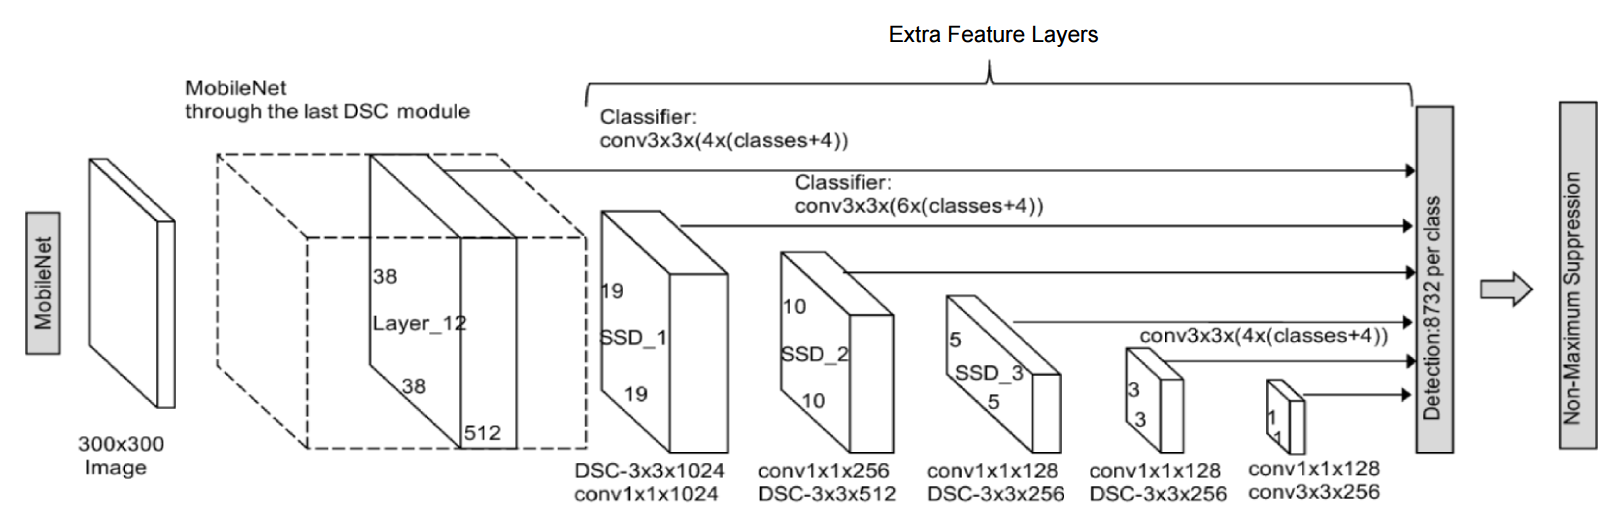
\includegraphics[width=1\textwidth]{figures/Diseno_global/ssd_mobilenet.png}
   \caption{Red \acrshort{ssd} Mobilenet V2}
	\label{fig.ssd_mobilenet}
\end{center}
\end{figure}

La primera parte de la red es la Mobilenet V2, en la cual se obtienen los mapas de características para poder realizar la clasificación y detección en las capas posteriores. 

\acrshort{ssd} ~\cite{ssd_article} es un método de detección de objetos en imágenes que emplea una única red neuronal profunda. \acrshort{ssd} proporciona una gran ganancia de velocidad frente a Faster \acrshort{rcnn} \cite{rcnn_faster}, que funciona a una tasa de 7 fotogramas por segundo. El enfoque de \acrshort{ssd} se basa en una red convolucional \textit{feed-forward} que produce un conjunto de \textit{bounding boxes} de tamaño fijo y puntúa la presencia de instancias de clase de objeto en esos \textit{bounding boxes}. Tras esto realiza \textit{non-maximum suppression} para producir las detecciones finales. 

Dada una imagen de entrada y un conjunto de etiquetas de \textit{ground truth}, \acrshort{ssd} realiza el siguiente proceso:
\begin{enumerate}
\item La imagen pasa a través de una serie de capas convolucionales, produciendo varios conjuntos de mapas de características a diferentes escalas.
\item Para cada ubicación en cada uno de estos mapas de características, emplea un filtro convolucional de 3x3 para evaluar un pequeño conjunto de \textit{bounding boxes} por defecto.
\item Para cada \textit{bounding box} predice simultáneamente el desplazamiento del \textit{bounding box} y las probabilidades de clase.
\item Durante el entrenamiento hace que coincida el \textit{bounding box} del \textit{ground truth} con los \textit{bounding boxes} predichos según \textit{\acrfull{iou}}. El mejor \textit{bounding box} predicho se etiquetará como "positivo", junto con todos los demás \textit{bounding boxes} que tengan un ratio de \textit{Intersection over Union} con el \textit{ground truth} mayor de 0.5.
\end{enumerate}

\acrshort{ssd} parece sencillo, pero el entrenamiento tiene un desafío único. Clasificamos y estimamos \textit{bounding boxes} desde cada posición en la imagen, usando múltiples formas diferentes, en diferentes escalas. Como resultado, generamos un número mucho mayor de \textit{bounding boxes} que en otros modelos, y casi todos ellos se corresponden con ejemplos negativos. Esto introduce un desequilibrio significativo entre los ejemplos de entrenamiento positivos y negativos.

Para solucionar este desequilibrio \acrshort{ssd} hace dos cosas. En primer lugar, utiliza la \textit{\acrfull{nms}} para agrupar \textit{bounding boxes} muy superpuestos en un solo \textit{bounding box}. En otras palabras, si cuatro \textit{bounding boxes} de formas, tamaños, etc, similares contienen el mismo objeto, el \acrshort{nms} conservará el que tenga la mayor confianza y descartará el resto. En segundo lugar, el modelo usa una técnica llamada minería negativa para equilibrar las clases durante el entrenamiento. En la minería negativa dura, solo se utiliza un subconjunto de los ejemplos negativos (es decir, falsos positivos) en cada iteración de entrenamiento. \acrshort{ssd} mantiene una relación de 3:1 de negativos a positivos.


Mobilenet emplea unas capas llamadas \textit{depthwise separable convolutions} en lugar de capas convolucionales para la clasificación. En una capa convolucional se extrae información mediante \textit{kernels} que recorren toda la imagen. Estos \textit{kernels} necesitan tener la misma profundidad que la imagen para ser aplicados, es decir, si tenemos una imagen RGB necesitaremos 3 \textit{kernels}, uno por cada canal de color. Las capas \textit{depthwise separable convolutions} siguen un proceso diferente a las convolucionales: 

\begin{enumerate}
    \item Realizan la operación \textit{depthwise convolution}, en la cual se aplican \textit{kernels} de igual profundidad que la imagen. Cada \textit{kernel} se aplica en cada canal de color por separado.
    \item Se lleva a cabo la operación \textit{pointwise convolution} en la cual se aplica un \textit{kernel} de 1x1xprofundidad de la imagen, con lo que se obtendrá así un único canal.
\end{enumerate}

Finalmente estos \textit{kernel} se combinan para obtener una única imagen. 
Si por ejemplo tenemos una imagen de 10x10x3 y se aplican capas convolucionales con \textit{kernels} de 3x3x3 el resultado será una imagen de 8x8x1. Si queremos aplicar 5 \textit{kernels} en total tendremos 5 \textit{kernels} de tamaño 3x3x3 que se moverán por la imagen 8x8 posiciones.

\begin{equation}\label{convolucional_formula}
N^{\circ} operaciones = 5x3x3x3x8x8 = 8640
\end{equation}

En el caso de \textit{depthwise separable convolutions} primero se realizará la operación \textit{depthwise convolution} con la cual obtendremos una imagen de 8x8x3 . Es decir, se emplearán 3 \textit{kernels} de tamaño 3x3x1 para cada canal de color y estos \textit{kernels} se moveran 8x8 posiciones. Tras esto se aplicará la operación \textit{pointwise convolution}, en la cual se usará un \textit{kernel} de tamaño 1x1x3 para obtener finalmente una imagen de 8x8x1. Si tuvieramos 5 \textit{kernels} de tamaño 1x1x3 se moverían 8x8 posiciones.

\begin{equation}\label{mobilenet_formula}
N^{\circ} operaciones = (3x3x3x1x8x8) + (5x1x1x3x8x8) = 2688
\end{equation}

En conclusión, las capas \textit{depthwise separable convolutions} realizan el mismo trabajo que las convolucionales pero lo dividen en dos, consiguiendo asi reducir el número de operaciones.

Con el diseño que se ha explicado se ha entrenado un total de 3173 imágenes, de las cuales 2700 eran de \textit{train} y 473 de validación. Las imágenes de \textit{train} son las que se usan para generar el modelo. Los datos de validación seleccionan el modelo que mejores resultados obtiene.

 \subsection{Entorno Keras y red SSD VGG-16}\label{sub.keras}
 
 Con \textit{Keras} se ha implementado una red \acrshort{ssd}. Para ello se ha recurrido al diseño realizados por Pierluigi Ferrari~\cite{ssd_ferrari}, el cual define una red \acrshort{ssd} que tiene como red base una VGG-16. En la Figura ~\ref{fig.ssd_300} se puede ver el diseño.
 
 \begin{figure}[H] 
\begin{center}
	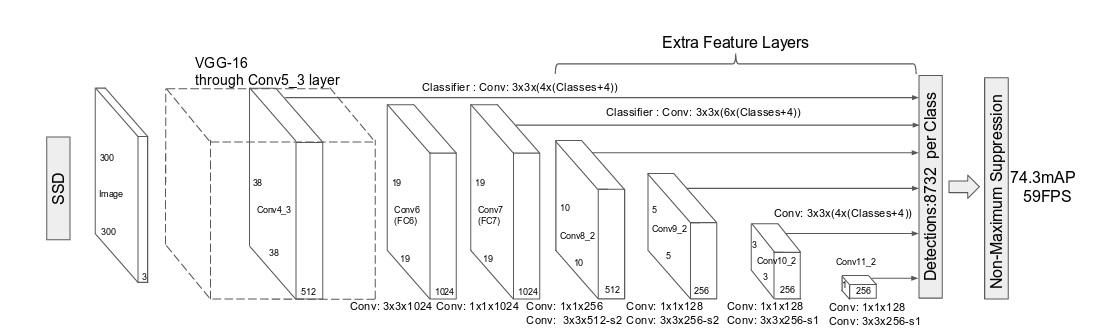
\includegraphics[width=1.1\textwidth]{figures/Diseno_global/ssd300.png}
   \caption{Red \acrshort{ssd}}
	\label{fig.ssd_300}
\end{center}
\end{figure}

VGG-16  está formada por 16 capas, de las cuales 13 son capas convolucionales, 2 capas totalmente conectadas y una capa de \textit{softmax} que se emplea para clasificar. En la Figura ~\ref{fig.vgg16} se puede ver cuál es la arquitectura de la red VGG-16.

 \begin{figure}[H] 
\begin{center}
	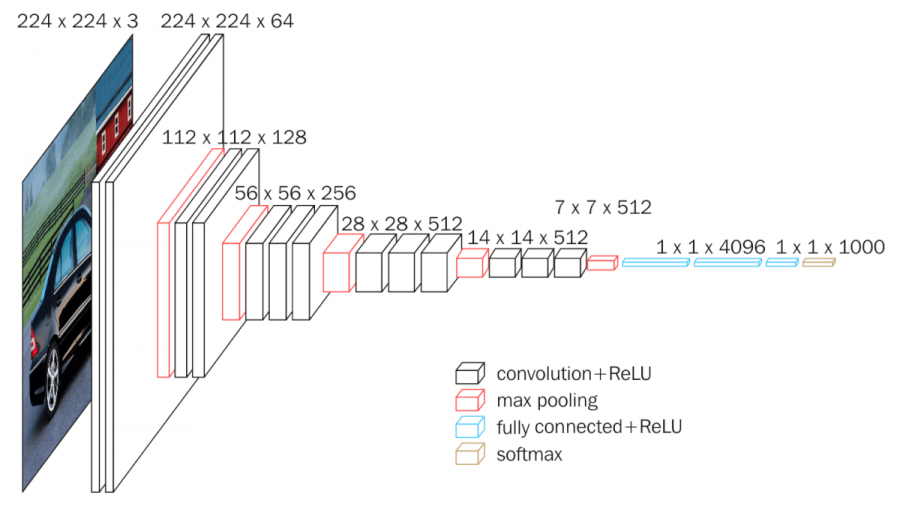
\includegraphics[width=0.8\textwidth]{figures/Diseno_global/vgg16.png}
   \caption{Red VGG-16}
	\label{fig.vgg16}
\end{center}
\end{figure}

\subsection{Entorno Darknet y red YOLOv3}\label{sub.darknet}

En este sistema se ha incluido \acrfull{yolo} debido a su gran éxito actualmente. \acrshort{yolo} ~\cite{yolo_article1} es otro enfoque para la detección de objetos. El trabajo previo a \acrshort{yolo} emplea clasificadores para realizar la detección. En esta aproximación se enmarca la detección de objetos como un problema de regresión en \textit{bounding boxes} espacialmente separados y probabilidades de clase asociadas. En la evaluación, una red neuronal única predice \textit{bounding boxes} y probabilidades de clase directamente desde imágenes completas. 

\acrshort{yolo} impone fuertes restricciones espaciales en las predicciones de los \textit{bounding boxes}, ya que cada celda de la cuadrícula solo predice N \textit{bounding boxes} (siendo N un parámetro fijo) y solo puede tener una clase. Esta restricción espacial limita el número de objetos cercanos que nuestro modelo puede predecir. En la Sección~\ref{sec.yolo} del Capítulo~\ref{cap.herramientas} se explica un poco \acrshort{yolo}.

La red Yolov3 está formada por un total de 107 capas,  las cuales se pueden agrupar en dos grupos, uno encargado de la extracción de características y otro de la detección de objetos:

\begin{itemize}
    \item Extracción de características (de la capa 1 a la 75): se trata de la red Darknet-53 entrenada con ImageNet, la cual se compone de 53 capas convolucionales (Figura~\ref{fig.darknet53}).
    \begin{figure}[H] 
\begin{center}
	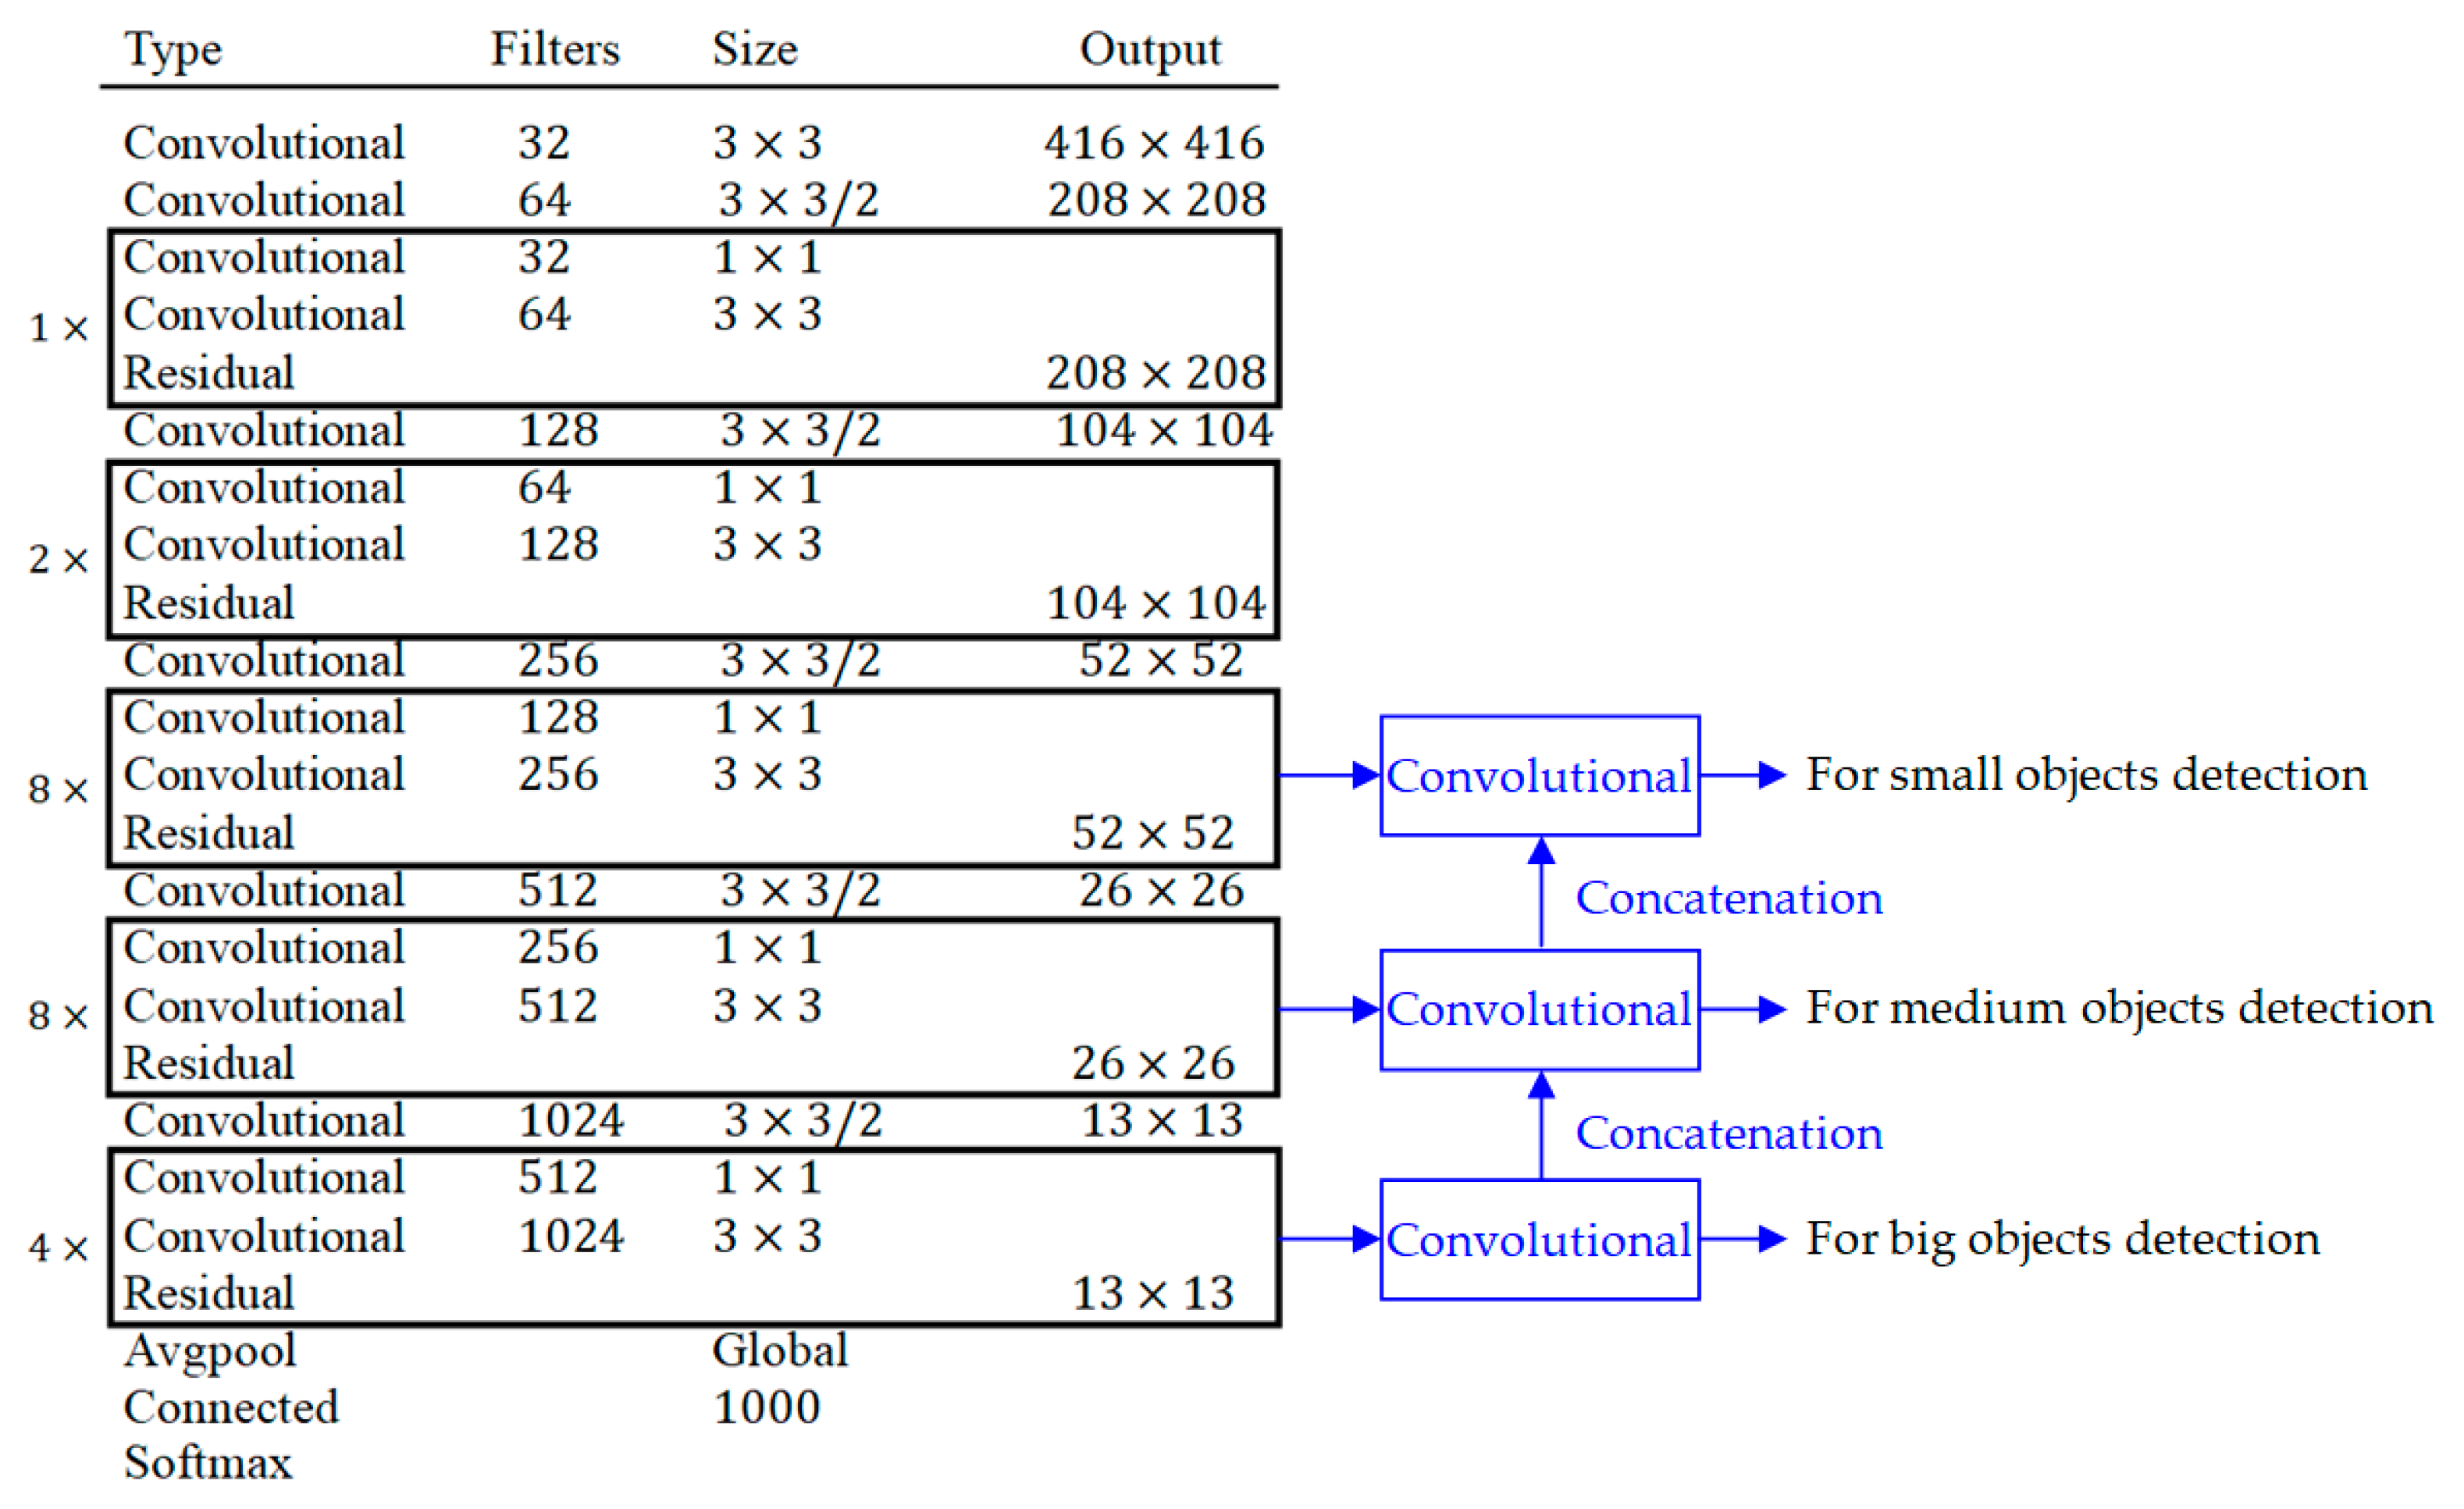
\includegraphics[scale=1]{figures/Diseno_global/darket53.png}
   \caption{Arquitectura Darknet-53}
	\label{fig.darknet53}
\end{center}
\end{figure}
	Esta red tiene como entrada imágenes de 416x416x3 y como salida características 3D de 13x13x1024, e incorpora 23 capas residuales. Cuando una red neuronal aumenta de profundidad su precisión a la hora de propagar las características tiende a degradarse llevándonos a un mayor error en el entrenamiento. Para solucionar este problema se hace uso de las capas residuales.
    \item Detección de Objetos (de la capa 76 a la 107): toma como entrada las características 3D (13x13x1024) y realiza con ello la detección de objetos. La singularidad de esta red reside en su capacidad para lograr detectar objetos en tres escalas diferentes, haciendo de ella una red muy potente ante el cambio de escala. Para ello extrae características en tres escalas diferentes (13x13x39, 26x26x39 y 52x52x39). Estas características pasan a la capa final YOLO, que clasifica la etiqueta del objeto con regresiones logísticas de clase y localiza los objetos con regresores de \textit{bounding boxes}.

\end{itemize}


La arquitectura unificada de \acrshort{yolo}v3 (Figura~\ref{fig.yolov3}) es extremadamente rápida, procesando imágenes en tiempo real a 30 fotogramas por segundo. Una versión más pequeña de la red, Fast \acrshort{yolo}, procesa 155 fotogramas por segundo, logrando duplicar el \textit{\acrfull{map}} de otros detectores en tiempo real.

\begin{figure}[H] 
\begin{center}
	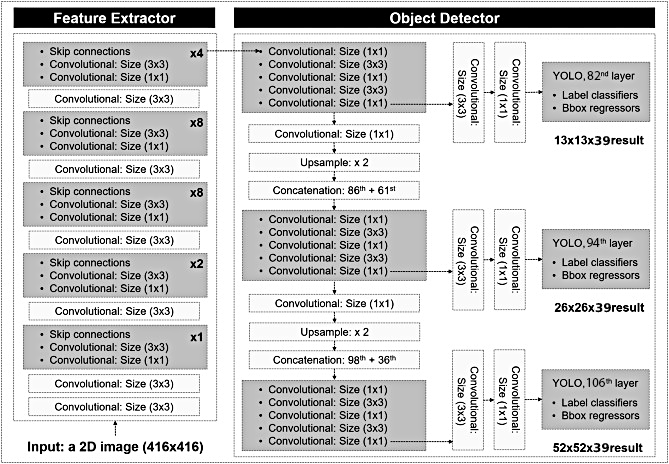
\includegraphics[scale=0.7]{figures/Diseno_global/yolov3.png}
   \caption{Arquitectura YOLOv3}
	\label{fig.yolov3}
\end{center}
\end{figure}

En comparación con los sistemas de detección más modernos, YOLO comete más errores de localización (especialmente con objetos pequeños), pero es menos probable que prediga falsos positivos en el fondo. \acrshort{yolo} aprende representaciones muy generales de objetos y supera a otros métodos de detección, como DPM y \acrshort{rcnn}, en imágenes naturales y trabajos artísticos.


\section{Seguimiento de Vehículos}\label{sec.seguimiento}

Una vez tenemos los vehículos detectados y clasificados debemos realizar su seguimiento a lo largo de la carretera. Es decir, tenemos que asociar cada \textit{blob} detectado a los \textit{blob} anteriores de los que ya se llevaba un seguimiento. El algoritmo empleado para realizar este \textit{tracking} está basado en la proximidad espacial y \acrshort{klt}. 

\subsection{Emparejamiento por proximidad}

La diferencia de píxeles en la imagen entre la posición de un vehículo en \textit{t-1} y en \textit{t} es muy pequeña. Por tanto se puede decir que el \textit{blob} de un vehículo en \textit{t} cae en una zona muy cercana al \textit{blob} de ese mismo vehículo en \textit{t-1}. Esto se tendrá en cuenta a la hora de realizar el seguimiento, ya que cuando busquemos un vehículo en \textit{t} deberíamos encontrarlo en un radio circular pequeño alrededor de la posición de ese mismo vehículo en \textit{t-1}. 

El algoritmo que se plantea en cuanto a la proximidad espacial es el empleado por Redouane Kachach en la versión anterior de la aplicación~\cite{redo_tesis}. En él se estima el área donde debería localizarse un vehículo en función de su posición en \textit{t-1}. A medida que los vehículos vayan avanzando este área se irá actualizando.

Al principio el área se toma como un círculo, pues no tenemos suficientes datos acerca de su orientación. Pero a medida que el vehículo avanza y tenemos suficiente información para conocer su orientación tomaremos el área como una elipse cuyo centro se corresponde con el centro del vehículo en \textit{t-1}. 

Consideraremos que tenemos suficiente información para estimar su orientación cuando tengamos 6 posiciones de un vehículo. Se emplea regresión lineal para calcular la orientación del vehículo basándonos en la posición que va tomando el vehículo a medida que va avanzando. 

La regresión lineal consiste en minimizar $\sum_{i}\rho(r_i)$ , donde $r_i$  es la  distancia  con  el  i-ésimo  punto  y $\rho(r_i)$ es una función de la distancia. $\rho(r_i)$ se puede calcular como:

\begin{equation}\label{ec.regresion_lineal}
   \rho(r_i) = 2(\sqrt{1 +\frac{r^2}{2}} - 1) 
\end{equation}

Una vez tenemos información acerca de la orientación definiremos el área de búsqueda como una elipse que tiene como centro el mismo que el vehículo en \textit{t-1} y dirección la calculada con la Fórmula (\ref{ec.regresion_lineal}).

Los emparejamientos entre los vehículos detectados en el instante \textit{t} y los \textit{blobs} almacenados del instante \textit{t-1} se limitan a los vehículos que caen dentro del área del círculo o la elipse que se obtiene en función de la posición del vehículo en el instante \textit{t-1}. En la Figura~\ref{fig.area_vehiculo} se puede ver la evolución que sufre el área alrededor del vehículo a medida que avanza.

 \begin{figure}[H] 
\begin{center}
	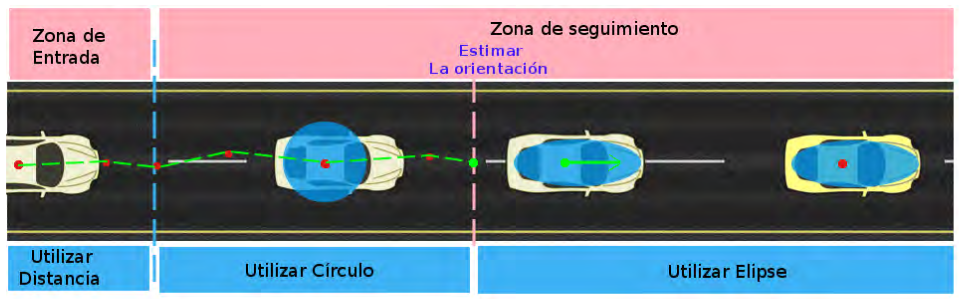
\includegraphics[width=0.9\textwidth]{figures/Diseno_global/areas_vehiculo.png}
   \caption{Evolución del área alrededor del vehículo}
	\label{fig.area_vehiculo}
\end{center}
\end{figure}


Estas elipses de definen como $C_{xc,yc,\omega}$, donde $\omega$ es la orientación y $(x_c, y_c)$ es el centro del vehículo. Además a la hora de describir una elipse debemos conocer sus dos ejes. Estos parámetros se pueden ver en la Figura ~\ref{fig.elipse}.

 \begin{figure}[H] 
\begin{center}
    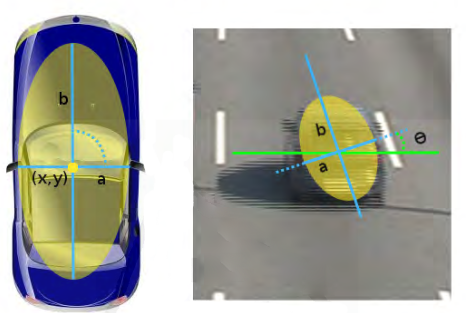
\includegraphics[width=0.7\textwidth]{figures/Diseno_global/elipse.png}
   \caption{Elipse asociada a los vehículos}
	\label{fig.elipse}
\end{center}
\end{figure}

Un blob 2D cuyo centro es $B(x,y)$ se encontrará dentro de la elipse  $C_{xc,yc,\omega}$ si se cumple:

\begin{equation}\label{ec.blob_elipse}
   C_{\omega} = \arctan(\frac{a_x}{a_y})
\end{equation}

\begin{equation} \scriptsize \label{ec.blob_elipse1}
   \left(\frac{cos(C_\omega)(B_x - C_{x_c}) + sin(C_\omega)(B_y - C_{y_c})}{a} \right)^2 + \left(\frac{cos(C_\omega)(B_y - C_{y_c}) - sin(C_\omega)(B_x - C_{x_c})}{b} \right)^2 \leq 1
\end{equation}

$a_x$ y $a_y$ son los componentes del vector de orientación. En la Figura ~\ref{fig.emparejamiento_blob} se puede ver cómo se realiza el \textit{tracking} entre dos \textit{blobs} consecutivos. 

 \begin{figure}[H] 
\begin{center}
   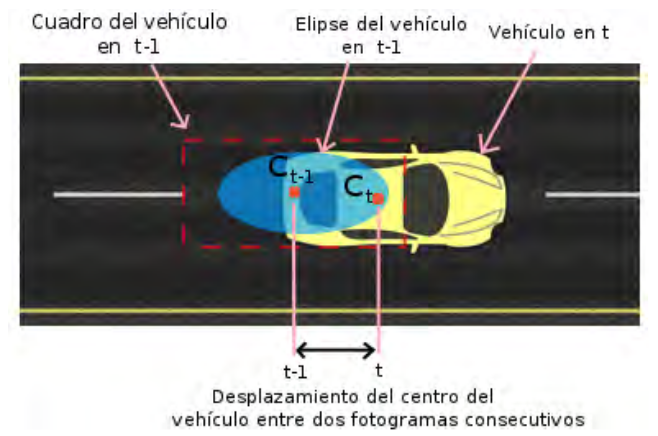
\includegraphics[width=0.7\textwidth]{figures/Diseno_global/emparejamiento_blob.png}
   \caption{Seguimiento con proximidad espacial}
	\label{fig.emparejamiento_blob}
\end{center}
\end{figure}


En la Figura~\ref{fig.proximidad_espacial} se muestra un ejemplo de \textit{Smart-Traffic-Sensor} donde se ve como se realiza el seguimiento de dos vehículos con proximidad espacial. El vehículo identificado como 2 en la imagen del instante t-1 se asocia al vehículo que se encuentra más cercano a su posición en la imagen del instante t. Lo mismo ocurre con el vehículo 3.

 \begin{figure}[H] 
\begin{center}
   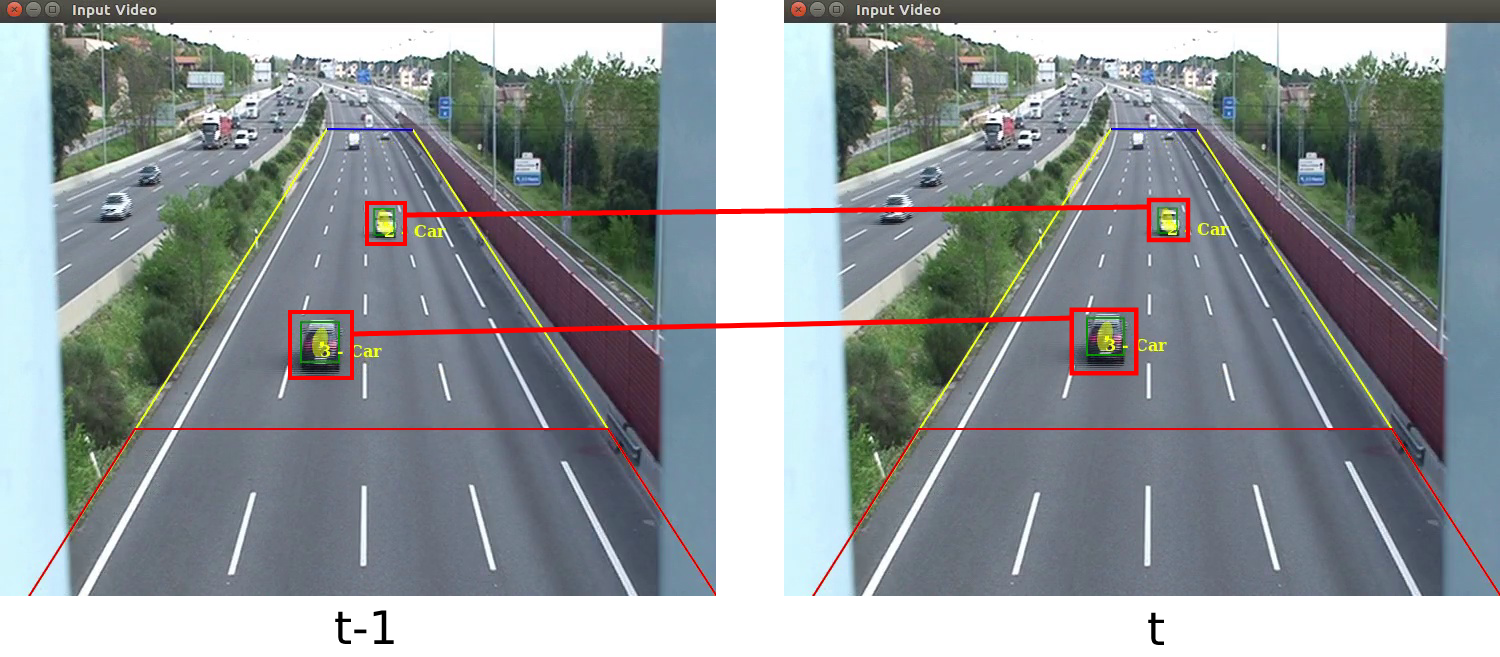
\includegraphics[scale=0.3]{figures/Diseno_global/proximidad_espacial.png}
   \caption{Seguimiento con proximidad espacial \textit{Smart-Traffic-Sensor}}
	\label{fig.proximidad_espacial}
\end{center}
\end{figure}

En resumen, una detección deberá encontrarse dentro de un cierto área alrededor del \textit{blob} detectado en \textit{t-1} para poder ser identificado como el mismo vehículo. Podría darse el caso de que dos vehículos cayeran en dicho área. Por ello es necesario tener en cuenta la distancia euclídea entre el centro del \textit{blob} del instante \textit{t-1} y el centro de los \textit{blob} en \textit{t}. Aquel \textit{blob} del instante \textit{t} que se encuentre a menor distancia del \textit{blob} del instante \textit{t-1} y por supuesto esté dentro del área alrededor del \textit{blob} \textit{t-1} será considerado como el mismo vehículo que el de \textit{t-1}. Es decir si esto se cumple el \textit{blob} de \textit{t-1} y \textit{t} corresponden al  mismo vehículo pero en instantes consecutivos.

\subsection{Seguimiento por KLT}

El seguimiento se centra en asociar las detecciones actuales con los \textit{blobs} almacenados del instante anterior. En el seguimiento se tendrán ciertos aspectos en cuenta:

\begin{itemize}
    \item Si un \textit{blob} llega al final de la zona de evaluación se eliminará del seguimiento.
    \item Se recorrerán los \textit{blob} del instante \textit{t-1} almacenados con el fin de emparejarlos con los \textit{blob} detectados en el instante \textit{t}. Este emparejamiento se establecerá entre los \textit{blobs} en \textit{t} y \textit{t-1} que tengan menor distancia euclídea entre sus centros.
    \item Si el \textit{blob} \textit{t} asociado al \textit{blob} \textit{t-1} no cae dentro del área circular o elíptica que se genera alrededor del centro del  \textit{blob} \textit{t-1} no quedará emparejado a éste. 
    \item Si mediante proximidad espacial no somos capaces de emparejar un \textit{blob} \textit{t-1} emplearemos \acrshort{klt}.
\end{itemize}

El seguimiento se basa principalmente en la proximidad espacial pero se hará uso de \acrshort{klt} en casos problemáticos, haciendo asi más robusto nuestro sistema. \acrshort{klt} se calculará en todas las secuencias para ir actualizando los puntos característicos.

Si no se detecta un vehículo ya sea porque haya alguna oclusión o se encuentre muy lejos, se empleará \acrshort{klt}, pues se ha visto que funciona incluso ante oclusiones durante un pequeño número de fotogramas consecutivos.

Para poder realizar \acrshort{klt} necesitamos conocer el centro de masas de los vehículos y sus características visuales. En función de los puntos característicos del vehículo en \textit{t-1}, \acrshort{klt} calcula el emparejamiento para cada punto característico y como resultado genera un nuevo conjunto de puntos característicos correspondientes al vehículo en cuestión. Para llegar a conseguir un emparejamiento correcto el sistema se basa en votos de los puntos característicos que un objeto tiene asociado. 

Un ejemplo del seguimiento mediante \acrshort{klt} se puede ver en la Figura~\ref{fig.klt_deteccion}. En ella se puede ver como a pesar de haber una oclusión se sigue detectando el vehículo. En este caso \textit{Deep Learning} no era capaz de detectarlo, pero gracias al uso de \acrshort{klt} no llegamos a perderlo.

 \begin{figure}[H] 
\begin{center}
   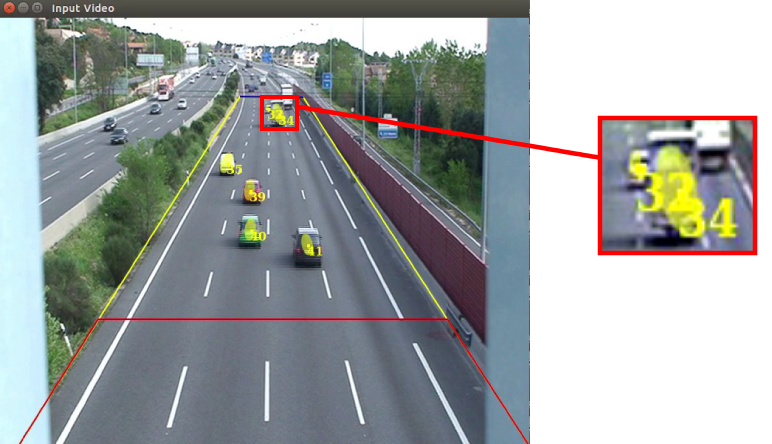
\includegraphics[scale=0.5]{figures/Diseno_global/klt_deteccion.png}
   \caption{Seguimiento con KLT \textit{Smart-Traffic-Sensor}}
	\label{fig.klt_deteccion}
\end{center}
\end{figure}

A continuación se va a explicar más en detalle \acrshort{klt}.

Jean-Yves Bouguet~\cite{klt_bouguet} hicieron una implementación de \acrshort{klt} en la cual aplicaban \acrshort{klt} de forma recursiva sobre una pirámide de imágenes. Esta misma implementación es la que se ha empleado en este trabajo. 

Lukas Kanade es un método diferencial y local en el que se analiza la vecindad de cada píxel. En él se asume que el flujo óptico es constante en una vecindad, y se resuelve la ecuación del flujo óptico para todos los píxeles en esta vecindad por el método de los mínimos cuadrados. Para el cálculo de los vectores de velocidad se emplea la siguiente fórmula:

\begin{equation}\label{klt_formula}
   \begin{bmatrix}u \\ v\end{bmatrix} = \begin{bmatrix}
            \sum_{i}I_{xi}^2 & \sum_{i}I_{xi}I_{yi} \\
            \sum_{i}I_{xi}I_{yi} &  \sum_{i}I_{yi}^2 \\
\end{bmatrix}^{-1} \begin{bmatrix}
-\sum_{i}I_{xi}I_{ti} \\
-\sum_{i}I_{yi}I_{ti} \\
\end{bmatrix}
\end{equation}
\\

El vector $(u,v)$ es el vector de desplazamiento del flujo óptico.
$I_x$ es la media del gradiente en x entre dos imágenes consecutivas, es decir, si $I(t)$ es la imagen del instante actual e $I(t+1)$ es la imagen en el instante siguiente, la $I_x$ de estos fotogramas es:

\begin{equation}
    I_x = \frac{I_x(t)+I_x(t+1)}{2}
\end{equation}

$I_x(t)$ es el gradiente en el eje x de la imagen $I(t)$ e $I_x(t+1)$ es el gradiente en $x$ de la imagen $I(t+1)$. $I_y$ es la media de los gradientes en $y$ de la imagen $I(t)$ e $I(t+1)$:

\begin{equation}
    I_y = \frac{I_y(t)+I_y(t+1)}{2}
\end{equation}

$I_t$ es la diferencia entre $I(t)$ suavizada e $I(t+1)$ suavizada:

\begin{equation}
   I_t = I'(t+1) - I'(t) 
\end{equation}

Tal y como se ha dicho \acrshort{klt} se aplica en forma de \textit{kernels} de tamaño $\omega x \omega$ a lo largo de la imagen. El tamaño de los \textit{kernels} debe ser definido en función de la cantidad de movimiento que tenga la imagen. Un valor de \textit{kernel} pequeño será idóneo para evaluar desplazamientos pequeños de un punto. El uso de un tamaño grande de \textit{kernel} aumenta el riesgo de obtener un error, pero hay en casos en los que el desplazamiento de un punto es muy grande y esto es necesario.

En la Figura ~\ref{fig.klt_piramidal} se puede ver cómo funciona \acrshort{klt} de forma piramidal.

 \begin{figure}[H] 
\begin{center}
	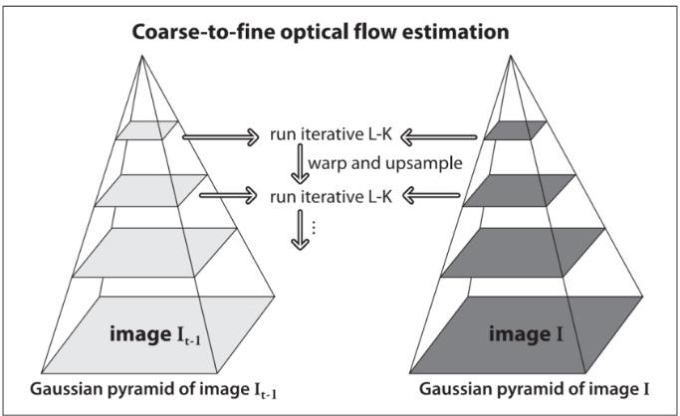
\includegraphics[width=0.7\textwidth]{figures/Diseno_global/klt_piramidal.png}
   \caption{\acrshort{klt} Piramidal}
	\label{fig.klt_piramidal}
\end{center}
\end{figure}

Gracias al empleo de \acrshort{klt} piramidal se pueden estimar grandes desplazamientos con un tamaño de ventana muy pequeño.


\section{Estimación de la Velocidad}

Gracias al seguimiento de vehículos, \textit{Smart-Traffic-Sensor} ofrece la funcionalidad de estimar la velocidad media que tienen estos vehículos durante su seguimiento.

\textit{Smart-Traffic-Sensor} tiene opciones para configurar la cámara, es decir para realizar su calibración. Al tener información de la cámara empleada tendremos información 3D de la imagen. Es decir podemos realizar una proyección al mundo 3D de nuestros puntos en la imagen.

Para calcular la velocidad sólo necesitamos conocer la distancia que ha recorrido el vehículo y el tiempo que ha tardado en hacerlo. Disponemos de una zona de evaluación por la cual discurren los vehículos, por tanto podemos saber cuánta distancia recorren por dicha zona de evaluación, y el tiempo que tardan en hacerlo. Para calcular la distancia tenemos que calcular la posición 3D de los vehículos y con ella hacer su diferencia. Esto se puede llevar a cabo haciendo uso de su homografía, la cual podemos estimar gracias a que conocemos los parámetros de la cámara.

\section{Interfaz Gráfica de la Aplicación}

La interfaz gráfica del proyecto nos da información en todo momento acerca de lo que sucede en el vídeo que estamos monitorizando, además de mostrarnos un histórico de la cantidad de vehículos que hemos procesado.

Esta interfaz gráfica tiene dos partes principales:
\begin{itemize}
    \item Una ventana denominada \textit{Input Video} en la que se ve el vídeo que evaluamos y su monitorizacion (detecciones, clasificación y seguimiento). Un ejemplo de esta ventana puede verse en la Figura~\ref{fig.input_video}.
     \begin{figure}[H] 
    \begin{center}
    	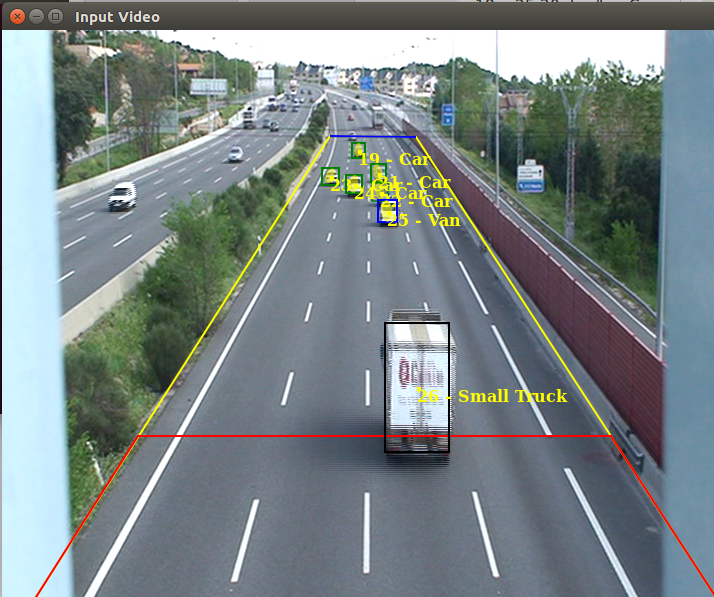
\includegraphics[scale=0.4]{figures/Diseno_global/sts_buena.png}
       \caption{Ventana \textit{Input Video}}
    	\label{fig.input_video}
    \end{center}
    \end{figure}
    \item La interfaz llamada \textit{Smart-Traffic-Sensor}, la cual controla toda nuestra aplicación y nos muestra información acerca de lo que se va registrando de la monitorización. Dicha ventana se puede ver en la Figura~\ref{fig.interfaz_sts}.
     \begin{figure}[H] 
    \begin{center}
    	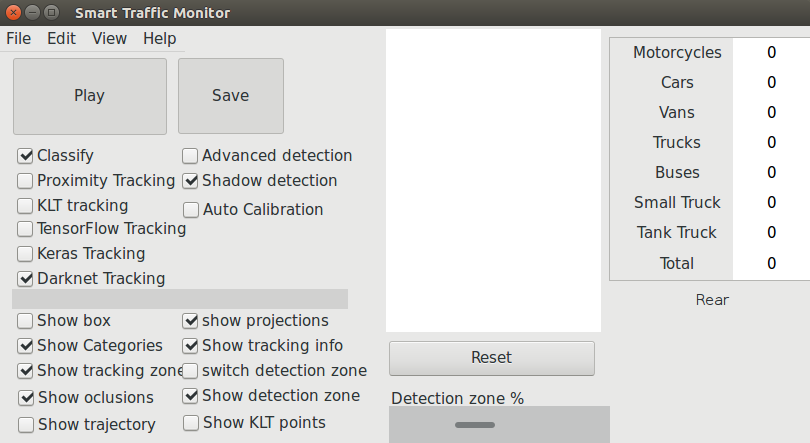
\includegraphics[scale=0.5]{figures/Diseno_global/interfaz_grafica.png}
       \caption{Interfaz \textit{
       Smart-Traffic-Sensor}}
    	\label{fig.interfaz_sts}
    \end{center}
    \end{figure}
\end{itemize}

La interfaz \textit{Smart-Traffic-Sensor} nos ofrece diversas funcionalidades para modificar lo que se muestra en la ventana \textit{Input Video}, nos permite cambiar el método de detección, clasificación y seguimiento, además de mostrarnos información acerca de los vehículos que se están monitorizando.

A continuación se va a explicar brevemente la funcionalidad de los botones que aplican en nuestro método, pues algunos solo aplican al funcionamiento del antiguo \textit{Traffic-Monitor}:
\begin{itemize}
    \item \textit{Play} permite detener y poner en marcha la ejecución del vídeo.
    \item \textit{Save} nos ofrece la posibilidad de guardar información acerca de la zona de evaluación, es decir, guardar información acerca del tamaño y los puntos en los que se encuentra la zona de evaluación.
    \item \textit{Classify} muestra los \textit{blobs} y su clase (siempre que esté también activo \textit{Show Categories}).
    \item \textit{Proximity Tracking}, \textit{KLT tracking}, \textit{TensorFlow Tracking}, \textit{Keras Tracking} y \textit{Darknet Tracking} permiten cambiar de método para la detección, clasificación y seguimiento. \textit{Proximity Tracking} y \textit{KLT tracking} pertenecen al algoritmo que desarrolló Redouane en su tesis~\cite{redo_tesis}. Con \textit{Proximity Tracking} se emplea únicamente proximidad espacial para el seguimiento y en \textit{KLT tracking} se incluye \acrshort{klt} para los casos en los que la detección es insuficiente. Con \textit{TensorFlow Tracking}, \textit{Keras Tracking} y \textit{Darknet Tracking} se activa el método desarrollado en este trabajo. La única diferencia entre ellos es la plataforma de detección y clasificación que se emplea.
    \item \textit{Show box} muestra el \textit{blob} completamente pintado de verde. Solo aplicará si no está activo \textit{Classify}. En la Figura~\ref{fig.show_box} se puede ver un ejemplo.
        \begin{figure}[H] 
    \begin{center}
    	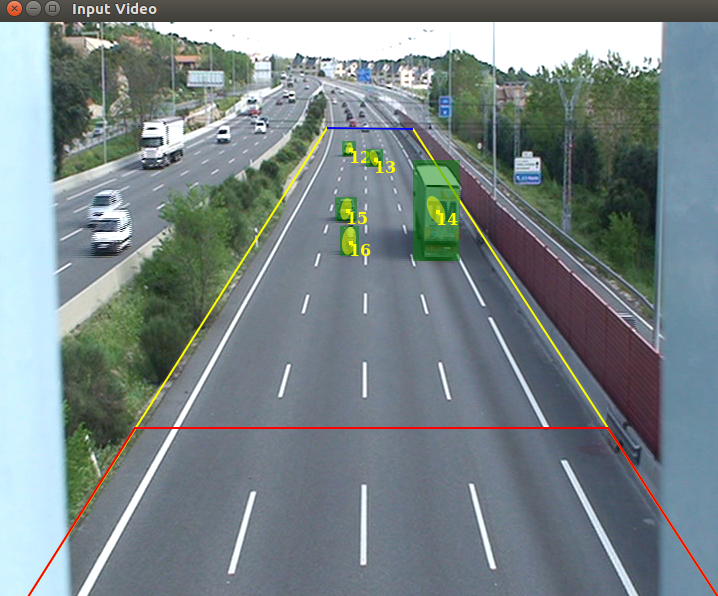
\includegraphics[scale=0.35]{figures/Diseno_global/show_box.png}
       \caption{\textit{Show box} activo}
    	\label{fig.show_box}
    \end{center}
    \end{figure}
    \item \textit{Show Categories} nos muestra la clase del vehículo monitorizado. Para que muestre la clase debe estar también activado \textit{Classify}.
    \item \textit{Show tracking zone} oculta o muestra la zona de evaluación.
    \textit{Show tracking info} nos permite ver en \textit{Input Video} toda la información de los vehículos monitorizados.
    \item \textit{Reset} inicializa todo el seguimiento de vehículos.
    \item \textit{Show trajectory} muestra la trayectoria que siguen los vehículos.
\end{itemize}

La interfaz también muestra un histórico de los vehículos monitorizados y una estadística total de la cantidad de vehículos de cada clase que han sido registrados. Esto puede verse en la Figura~\ref{fig.info_vehicles}.

    
Con todo ello tenemos una interfaz que nos muestra información acerca de los vehículos monitorizados muy completa.


    \begin{figure}[H] 
    \begin{center}
    	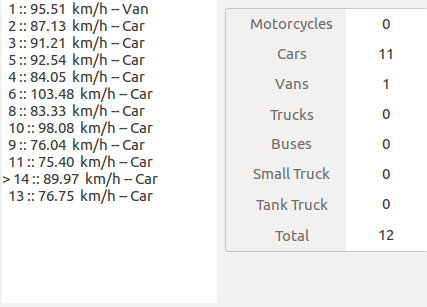
\includegraphics[scale=0.6]{figures/Diseno_global/info.png}
       \caption{Información de los Vehículos Monitorizados}
    	\label{fig.info_vehicles}
    \end{center}
    \end{figure}
    


